\documentclass[10pt]{standalone}
\usepackage[utf8]{inputenc}
\usepackage{pgf,tikz}
\usepackage{mathrsfs}
\usetikzlibrary{arrows,positioning,calc}
\pagestyle{empty}
\usepackage[T1]{fontenc} % font encoding
\usepackage[utf8]{inputenc} % input encoding
%\usepackage{noto}
\usepackage[largesc]{newtxtext} %
\usepackage[varqu,varl]{zi4}% inconsolata
\usepackage{cabin}% sans serif
\usepackage[vvarbb]{newtxmath}
\useosf % use oldstyle figures except in math

%\tikzset{every picture/.style={scale=0.3,every picture/.style={}}}
\tikzset{main base/.style={draw,thick,text centered, }, }
\tikzset{main node/.style={rectangle, draw,rounded corners,main base}, }
%      
%\tikzset{main verb/.style={minimum size=1cm}, }
%\tikzset{linea/.style={-triangle 90}, }
%\tikzset{main node2/.style={rectangle, draw,thick,
%    text width=7em, text centered, rounded corners, minimum height=3em}, }
\tikzset{main node2/.style={main node,
    text width=7em, minimum height=3em}, }
\tikzset{main verb/.style={minimum size=1cm}, }
\tikzset{linea/.style={-triangle 90,thick,draw}}
%\tikzset{linea/.style={-triangle 90,thick,draw}}
\tikzset{linea2/.style={-triangle 90,draw}}
\tikzset{primo/.style={circle,draw,inner sep=0pt,minimum size=1pt,thick}, }
\tikzset{
    start-end/.style={
        draw,
        rectangle,
        rounded corners,main base,
    } ,
    input/.style={ % requires library shapes.geometric
        draw,
        trapezium,
        trapezium left angle=60,
        trapezium right angle=120,main base
    },
    operation/.style={
        draw,thick,
        rectangle,main base,
    },
    loop/.style={ % requires library shapes.misc
        draw,
        chamfered rectangle,
        chamfered rectangle xsep=2cm
    },
    decision/.style={ % requires library shapes.geometric
        draw,
        diamond,
        aspect=#1,main base
    },
    decision/.default=1,
    print/.style={ % requires library shapes.symbols
        draw,
        tape,
        tape bend top=none
    },
    connection/.style={
        draw,
        circle,
        radius=5pt,
    },
    process rectangle outer width/.initial=0.15cm,
    predefined process/.style={
        rectangle,
        draw,
        append after command={
        \pgfextra{
          \draw
          ($(\tikzlastnode.north west)-(0,0.5\pgflinewidth)$)--
          ($(\tikzlastnode.north west)-(\pgfkeysvalueof{/tikz/process rectangle outer width},0.5\pgflinewidth)$)--
          ($(\tikzlastnode.south west)+(-\pgfkeysvalueof{/tikz/process rectangle outer width},+0.5\pgflinewidth)$)--
          ($(\tikzlastnode.south west)+(0,0.5\pgflinewidth)$);
          \draw
          ($(\tikzlastnode.north east)-(0,0.5\pgflinewidth)$)--
          ($(\tikzlastnode.north east)+(\pgfkeysvalueof{/tikz/process rectangle outer width},-0.5\pgflinewidth)$)--
          ($(\tikzlastnode.south east)+(\pgfkeysvalueof{/tikz/process rectangle outer width},0.5\pgflinewidth)$)--
          ($(\tikzlastnode.south east)+(0,0.5\pgflinewidth)$);
        }  
        },
        text width=#1,
        align=center
    },
    predefined process/.default=1.75cm,
    man op/.style={ % requires library shapes.geometric
        draw,
        trapezium,
        shape border rotate=180,
        text width=2cm,
        align=center,
    },
    extract/.style={
        draw,
        isosceles triangle,
        isosceles triangle apex angle=60,
        shape border rotate=90
    },
    merge/.style={
        draw,
        isosceles triangle,
        isosceles triangle apex angle=60,
        shape border rotate=-90
    },
}

\begin{document}
 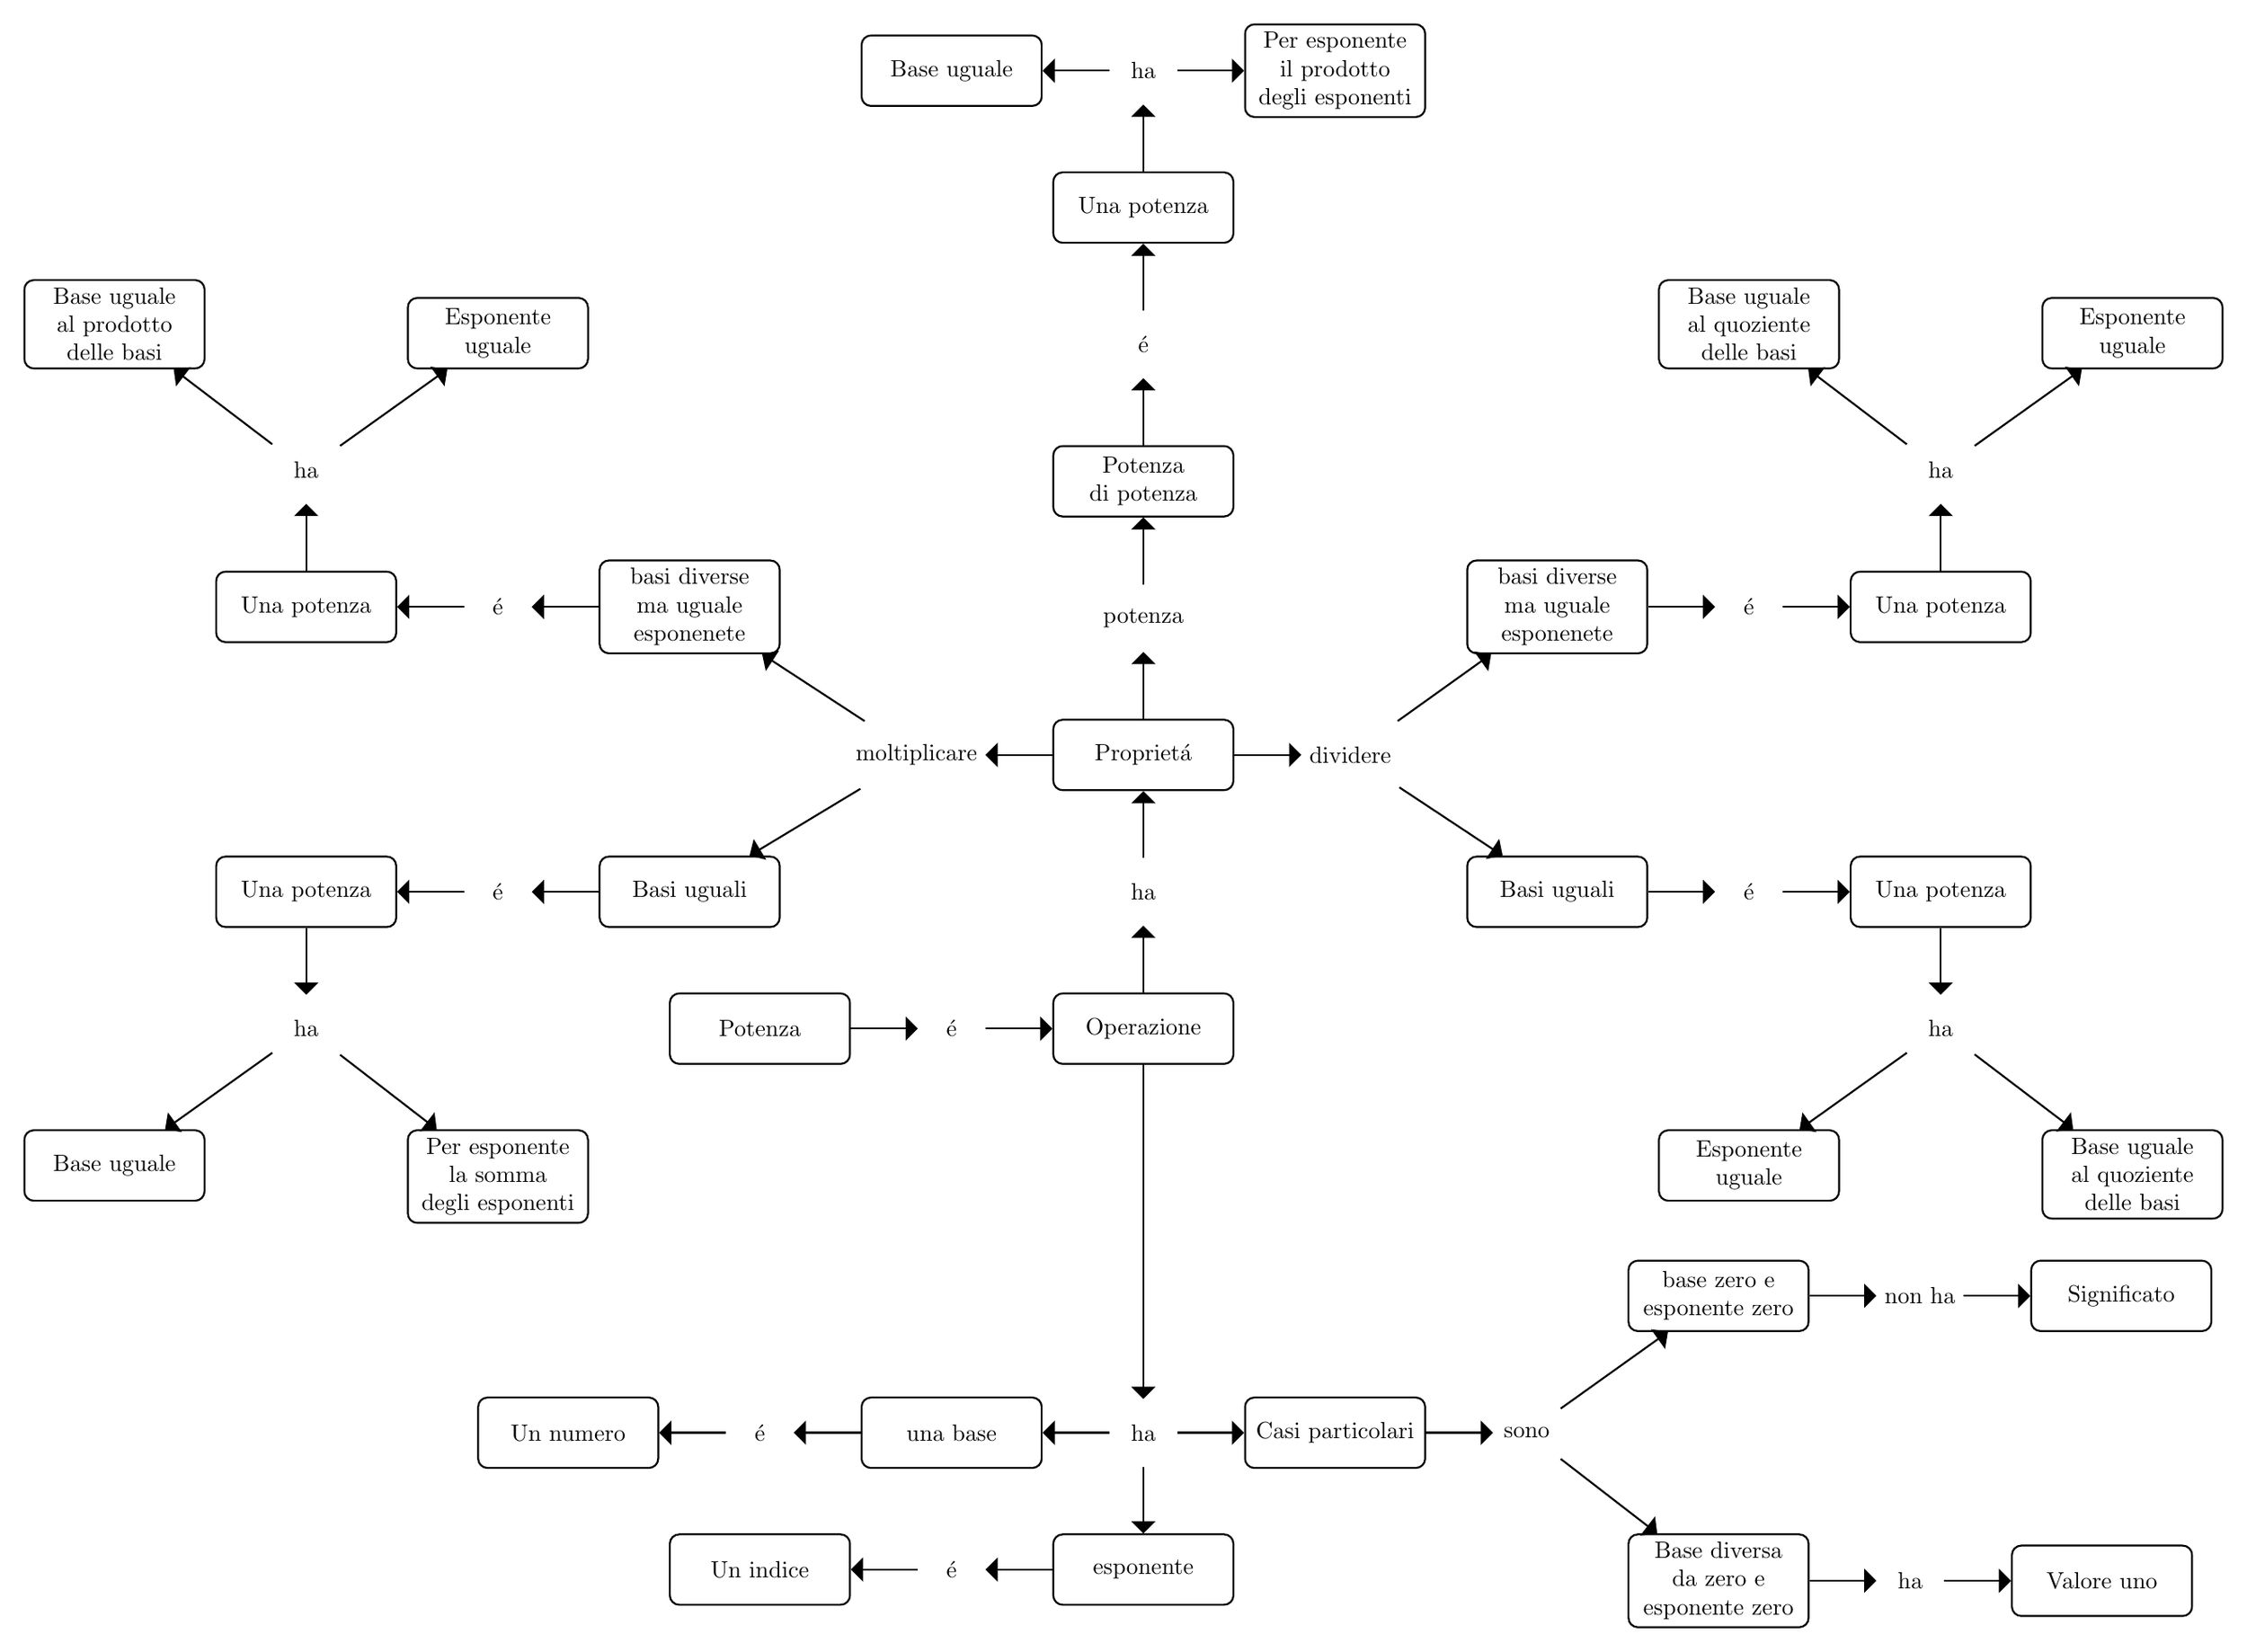
\begin{tikzpicture}
\tikzset{every picture/.style={scale=0.3,every picture/.style={}}}
\tikzset{main base/.style={draw,thick,text centered, }, }
\tikzset{main node/.style={rectangle, draw,rounded corners,main base}, }
%      
%\tikzset{main verb/.style={minimum size=1cm}, }
%\tikzset{linea/.style={-triangle 90}, }
%\tikzset{main node2/.style={rectangle, draw,thick,
%    text width=7em, text centered, rounded corners, minimum height=3em}, }
\tikzset{main node2/.style={main node,
		text width=7em, minimum height=3em}, }
\tikzset{main verb/.style={minimum size=1cm}, }
\tikzset{linea/.style={-triangle 90,thick,draw}}
%\tikzset{linea/.style={-triangle 90,thick,draw}}
\tikzset{linea2/.style={-triangle 90,draw}}
\tikzset{primo/.style={circle,draw,inner sep=0pt,minimum size=1pt,thick}, }
\tikzset{
	start-end/.style={
		draw,
		rectangle,
		rounded corners,main base,
	} ,
	input/.style={ % requires library shapes.geometric
		draw,
		trapezium,
		trapezium left angle=60,
		trapezium right angle=120,main base
	},
	operation/.style={
		draw,thick,
		rectangle,main base,
	},
	loop/.style={ % requires library shapes.misc
		draw,
		chamfered rectangle,
		chamfered rectangle xsep=2cm
	},
	decision/.style={ % requires library shapes.geometric
		draw,
		diamond,
		aspect=#1,main base
	},
	decision/.default=1,
	print/.style={ % requires library shapes.symbols
		draw,
		tape,
		tape bend top=none
	},
	connection/.style={
		draw,
		circle,
		radius=5pt,
	},
	process rectangle outer width/.initial=0.15cm,
	predefined process/.style={
		rectangle,
		draw,
		append after command={
			\pgfextra{
				\draw
				($(\tikzlastnode.north west)-(0,0.5\pgflinewidth)$)--
				($(\tikzlastnode.north west)-(\pgfkeysvalueof{/tikz/process rectangle outer width},0.5\pgflinewidth)$)--
				($(\tikzlastnode.south west)+(-\pgfkeysvalueof{/tikz/process rectangle outer width},+0.5\pgflinewidth)$)--
				($(\tikzlastnode.south west)+(0,0.5\pgflinewidth)$);
				\draw
				($(\tikzlastnode.north east)-(0,0.5\pgflinewidth)$)--
				($(\tikzlastnode.north east)+(\pgfkeysvalueof{/tikz/process rectangle outer width},-0.5\pgflinewidth)$)--
				($(\tikzlastnode.south east)+(\pgfkeysvalueof{/tikz/process rectangle outer width},0.5\pgflinewidth)$)--
				($(\tikzlastnode.south east)+(0,0.5\pgflinewidth)$);
			}  
		},
		text width=#1,
		align=center
	},
	predefined process/.default=1.75cm,
	man op/.style={ % requires library shapes.geometric
		draw,
		trapezium,
		shape border rotate=180,
		text width=2cm,
		align=center,
	},
	extract/.style={
		draw,
		isosceles triangle,
		isosceles triangle apex angle=60,
		shape border rotate=90
	},
	merge/.style={
		draw,
		isosceles triangle,
		isosceles triangle apex angle=60,
		shape border rotate=-90
	},
}
 \node[main node2] (1) {Potenza};
 \node[main verb] (2) [right=of 1] {\'{e}};
 \node[main node2] (3) [right=of 2] {Operazione};
 \node[main verb] (4) [above=of 3] {ha};
 %\node[main verb] (5) [below right=of 3] {ha}; 
 \node[main verb] (6) [below =5cm and 0cm of 3] {ha};
 \node[main node2] (7) [above= of 4] {Propriet\'{a}};
 
 \node[main node2] (8) [right= of 6] {Casi particolari};
 
 \node[main node2] (9) [left= of 6] {una base};
 
 \node[main node2] (10) [below = of 6] {esponente};

 \node[main verb] (11) [left= of 7] {moltiplicare};
 \node[main verb] (12) [above= of 7] {potenza}; 
 \node[main verb] (13) [right= of 7] {dividere};
 
 \node[main verb] (14) [right= of 8] {sono};
 \node[main verb] (15) [left= of 9] {\'{e}};
 \node[main verb] (16) [left= of 10] {\'{e}};
 
 \node[main node2] (17) [above left= of 11] {basi diverse ma uguale esponenete};
 \node[main node2] (18) [below left= of 11] {Basi uguali};
 
 \node[main node2] (19) [above= of 12] {Potenza di potenza};
 
 \node[main node2] (20) [above right= of 13] {basi diverse ma uguale esponenete};
 \node[main node2] (21) [below right= of 13] {Basi uguali};
 
 \node[main node2] (22) [above right=of 14] {base zero e esponente zero};
 \node[main node2] (23) [below right=of 14] {Base diversa da zero e esponente zero};
 \node[main node2] (24) [left= of 15] {Un numero};
 \node[main node2] (25) [left= of 16] {Un indice}; 
 
 \node[main verb] (26) [left=of 17] {\'{e}};
 \node[main verb] (27) [left=of 18] {\'{e}};
 \node[main verb] (28) [above=of 19] {\'{e}};
 \node[main verb] (29) [right=of 20] {\'{e}};
 \node[main verb] (30) [right=of 21] {\'{e}};
 \node[main verb] (31) [right =of 22] {non ha};
 \node[main verb] (32) [right=of 23] {ha};
 \node[main node2] (33) [left=of 26] {Una potenza};
 \node[main node2] (34) [left=of 27] {Una potenza};
 \node[main node2] (35) [above=of 28] {Una potenza};
 \node[main node2] (36) [right=of 29] {Una potenza};
 \node[main node2] (37) [right=of 30] {Una potenza};
 \node[main node2] (38) [right=of 31] {Significato};
 \node[main node2] (39) [right=of 32] {Valore uno};
 \node[main verb] (40) [above=of 33] {ha};
 \node[main verb] (41) [below=of 34] {ha};
 \node[main verb] (42) [above=of 35] {ha};
 \node[main verb] (43) [above=of 36] {ha};
 \node[main verb] (44) [below=of 37] {ha};
 \node[main node2] (45) [above left= of 40] {Base uguale al prodotto delle basi};
 \node[main node2] (46) [above right= of 40] {Esponente uguale}; 
 \node[main node2] (47) [below right= of 41] {Per esponente la somma degli esponenti };
 \node[main node2] (48) [below left= of 41] {Base uguale};
 
 \node[main node2] (49) [right=of 42] {Per esponente il prodotto degli esponenti };
 \node[main node2] (50) [left= of 42] {Base uguale};
\node[main node2] (51) [above right= of 43] {Esponente uguale };
 \node[main node2] (52) [above left= of 43] {Base uguale al quoziente delle basi};
\node[main node2] (53) [below left= of 44] {Esponente uguale };
 \node[main node2] (54) [below right= of 44] {Base uguale al quoziente delle basi};

\foreach \x /\y in{1/2,2/3,3/4,3/6,4/7,6/8,6/9,6/10,7/11,7/12,7/13,8/14,9/15,10/16,11/17,11/18,12/19,13/20,13/21,14/22,14/23,15/24,16/25,17/26,18/27,19/28,20/29,21/30,22/31,23/32,26/33,27/34,28/35,29/36,30/37,31/38,32/39,33/40,34/41,35/42,36/43,37/44,40/45,40/46,41/47,41/48,42/49,42/50,43/51,43/52,44/53,44/54}
 \path[linea] (\x) edge node {} (\y);
% 
\end{tikzpicture}
\end{document}